\section{Landmark-directed dimensionality reduction\label{sec:methods}}

EmbedSOM is a visualization-oriented method of non-linear dimensionality reduction that works by describing a high-dimensional point by its location relative to landmarks equipped with a topology and reproducing the point in a low-dimensional space using an explicit low-dimensional projection of the landmarks with the same topology~\cite{kratochvil2019generalized}.
% The ability to effectively work with a simplified model of the data differentiates it from other dimensionality reduction methods; in turn it offers superior performance by reducing the amount of necessary computation as well as by opening parallelization potential, since the computations of the projections of many individual points are independent.
% In the setting of flow and mass cytometry data visualization, this provided speedup of several orders of magnitude against the other available methods~\cite{kratochvil2020gigasom,kratochvil2020shinysom}.

% While the EmbedSOM originally used the (eponymous) self-organizing maps to find the viable high- and low-dimensional manifolds from the data points, the concept generalized well to many other methods.
% In particular, the projection has been shown to work with any (even random) set of high-dimensional landmarks that have the low-dimensional counterparts organized by any selected dimensionality reduction method (which may be slow in comparison, given the fact that the set of landmarks is usually small).
% In Section~\ref{ssec:dynamic}, we utilize this freedom of model specification to provide dynamic view of the dataset, based on a simplified dataset model that the user may refines in order to improve the dataset view.

More formally, the EmbedSOM algorithm works as follows. Let $d$ be the dimension of the high-dimensional space and assume $\mathbb{R}^2$ is the low-dimensional space for brevity. EmbedSOM processes $n$ $d$-dimensional points in a matrix $X$ of size $n\times d$, and outputs $n$ 2-dimensional points in matrix $x$ of size $n\times 2$.
The high- and low-dimensional landmarks similarly form matrices $L$ of size $g\times d$ and $l$ of size $g\times 2$, where usually $g\ll n$.
Each point $X_i$ is transformed to a point $x_i$ as:
\begin{enumerate}
\item $k$ nearest landmarks are found for point $X_i$ ($k$ is a constant parameter satisfying $3\leq k\leq g$)
\item the landmarks are ordered and a score is assigned to each of them, using a smooth function of the distance that assigns the highest score to the closest landmark and $0$ to the $k$-th landmark (this ensures the smoothness of projection in cases when $k<g$ \cite{kratochvil2019generalized})
\item for each pair $(u,v)$ of the closest $k-1$ landmarks (i.e., the ones with non-zero score), a projection of the point $X_i$ is found on the 1-dimensional affine space with coordinate 0 at $L_u$ and 1 at $L_v$; the 1-dimensional coordinate of the projection in this affine space is taken as $D_{uv}(X_i)$ and the same projected coordinates are defined in the low-dimensional space as $d_{uv}(x_i)$
\item point $x_i$ is fitted to the low-dimensional space so that the squared error in the coordinates weighed by nearest-landmark scores ($s_u, s_v$) is minimized: $$x_i = \argmin_{p\in \mathbb{R}^2} \sum_{u,v}s_u\cdot s_v\cdot \left(D_{uv}(X_i)-d_{uv}(p)\right)^2$$
\end{enumerate}

Because $d_{uv}(p)$ is designed as a linear operator, the error minimization problem (step 4) collapses to a trivial solution of $2$ linear equations with $2$ variables.
A complete algorithm may be found in the original publication~\cite[Algorithm 1]{kratochvil2019generalized}.

% Efficient implementation of the EmbedSOM algorithm is the main performance concern that enables its interactive use.
% The original CPU-based parallel implementation was able to visualize hundreds of thousands of points per second on common use-cases.
% As a major result of this paper, in Section~\ref{sec:impl} we improve this performance to the scale of milliseconds, enabling real-time projection and rendering of points based on interactive control of the high- and low-dimensional landmarks.

% \subsection{User supervision and model interaction}
% \label{ssec:dynamic}

% EmbedSOM landmarks (the matrices $L$ and $l$) represent a simplified dataset model that can be used to conveniently and predictably steer the dimensionality reduction.
% In particular, the main property of the projection --- visualizing the data points from the neighborhood of a landmark $L_i$ preferably in the neighborhood of the corresponding low-dimensional $l_i$ --- gives an intuitive interpretation for the landmark positions:
% Manipulating the high-dimensional landmarks chooses which data are visualized, while manipulating the low-dimensional landmarks chooses the desired location of the visualized points.
% Smoothness of the projection then grants that the smooth manipulations of the landmarks that will result in smooth changes of the results, enabling predictable user control and refinement.

% However, positioning of the landmarks in the high-dimensional space (which is inherently complicated to navigate) and finding a suitable layout of the landmarks in the low-dimensional space is an overly complicated task for the user alone.
% The main concern of this section is to design a simplification of the control of the landmarks, so that viable results may be reached in an automated way and the user interaction is required only for decisions that can not be decided automatically such as resolving dimensionality-reduction ambiguities and positioning of the dataset parts that matches some assumed semantics.
% We describe two ways of automated and user-controlled positioning of the landmarks that implement this kind of partial supervision, thus making the method semi-supervised.
% Both are roughly based on the embedding methods proposed in previous work~\cite{kratochvil2019generalized}; only modified for interactive environment.

% The main tasks that the user supervision interface has to resolve are thus as follows:
% \begin{itemize}
% \item place the landmarks to viable positions in the high-dimensional space
% \item dynamically increase or decrease the resolution of the model in specified places, by adding or removing landmarks
% \item organize low-dimensional landmarks to reflect the structure in the high-dimensional space, while allowing the user to resolve ambiguities that arise in dimensionality reduction
% \item react to the changes in the input datasets, such as scaling of the dimensions and appearance of new points
% \end{itemize}

% \begin{figure}
% \centering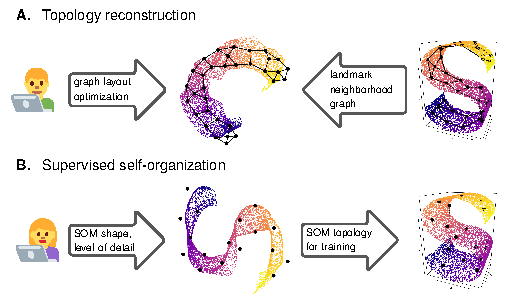
\includegraphics[width=\linewidth]{embedsom/pic/sup.pdf}
% \caption{
% Schema of the 2 implemented user supervision approaches.
% The user interacts with low-dimensional model that is intuitive to navigate, and indirectly drives the positioning of the corresponding high-dimensional image of the model, using either a graph-based approach (Section~\ref{sssec:sup-graph}) or self-organizing map approach (Section~\ref{sssec:sup-som}).
% }
% \label{fig:supervis}
% \end{figure}

% The two methods detailed below are briefly illustrated in Figure~\ref{fig:supervis}.

% \subsubsection{Semi-supervised structure reconstruction}
% \label{sssec:sup-graph}

% One possible approach to position the high-dimensional landmarks is to sample them randomly from the distribution of the original data set, and position the low-dimensional ones to reflect the structure of the sampling.
% In the original unsupervised implementation, we used a random sample of the input dataset as the landmark positions, and a dimensionality reduction methods such as t-SNE to position the landmarks.
% Importantly, the positioning of low-dimensional landmarks could be performed relatively quickly even by rather time-demanding algorithms such as t-SNE, because the algorithm only had to work with the highly reduced version of the dataset in landmarks.

% In the dynamic, supervised context, we need to avoid the randomness in order to avoid flickering in the view of the dataset, and utilize a dimensionality reduction algorithm that may reflect the user input.
% Thus, we chose to continuously run an interactive version of $k$-means clustering with a low learning rate to find good $k$ high-dimensional landmarks $L$, and employ a simple force-based graph layouting algorithm on a neighborhood graph of $L$ to embed the landmarks to 2D.
% Both these algorithms are capable of smooth transitions between consecutive states, thus avoiding the flicker.
% Moreover, force-based graph layouting may be intuitively steered by the user by dragging the graph nodes. Similarly, the points may be added and removed from $k$-means clustering in the same interface in order to increase and decrease the model resolution.

% Addition of a new landmark is implemented as follows: The user selects a low-dimensional landmark, and upon pressing a special button, both the low-dimensional landmark and its high-dimensional counterparts are duplicated in their respective spaces.
% The $k$-means algorithm then consecutively optimizes the positions of the landmarks to provide a detailed view.
% This stability of the result is helped by the initialization properties of $k$-means where the cluster centroids tend to stay in the same clusters~\cite{franti2019much} (counter-intuitively, the same properties have an undesirable impact on the robustness of unsupervised clustering).
% Most importantly, this enables the user to position new landmarks without having to navigate the possibly overwhelming complexity of the data distribution in the high-dimensional space.

% \subsubsection{Supervised training of self-organizing maps}
% \label{sssec:sup-som}

% Alternatively, the user may choose a SOM approach as originally intended for EmbedSOM.
% BlosSOM supports user drawing of the 2-dimensional version of the SOM on a canvas, which is used as-is as the low-dimensional landmarks.
% New landmarks may be added at any position, as their initial high-dimensional coordinates can be fitted using the coordinates of the other close landmarks in 2D.

% The positioning of the landmarks in 2D is then used as a topology for training the high-dimensional landmarks as neuron weights of the SOM algorithm.
% To extend the supervision possibilities of this step, BlosSOM adds specific controls that allow the user to manually sweep through the SOM neighborhood sizes and learning rates (usually labeled $\sigma$ and $\alpha$ \cite{kohonen1990self}), which is done automatically in unsupervised SOM training.
% This allows the users to optionally pause the SOM training at any stage and fix or customize the SOM topology at coarse detail level (with larger $\sigma$) before it is used to train fine details (small $\sigma$, the difference is closer detailed in Figure~\ref{fig:somsigma}).

% \begin{figure}
% \centering
% \begin{tikzpicture}[node distance=1em]
% \node (a) {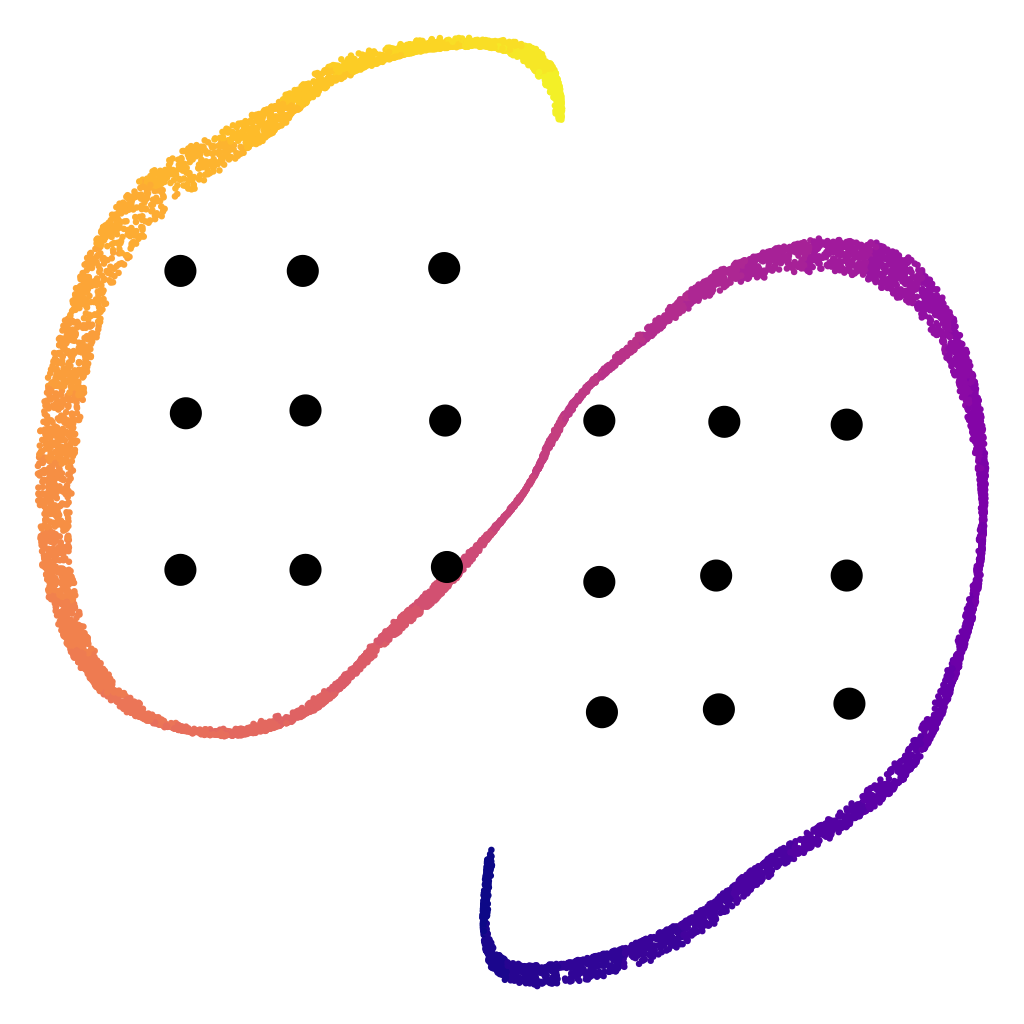
\includegraphics[width=.25\linewidth]{embedsom/pic/S_begin_2d.png}};
% \node[right=of a] (b) {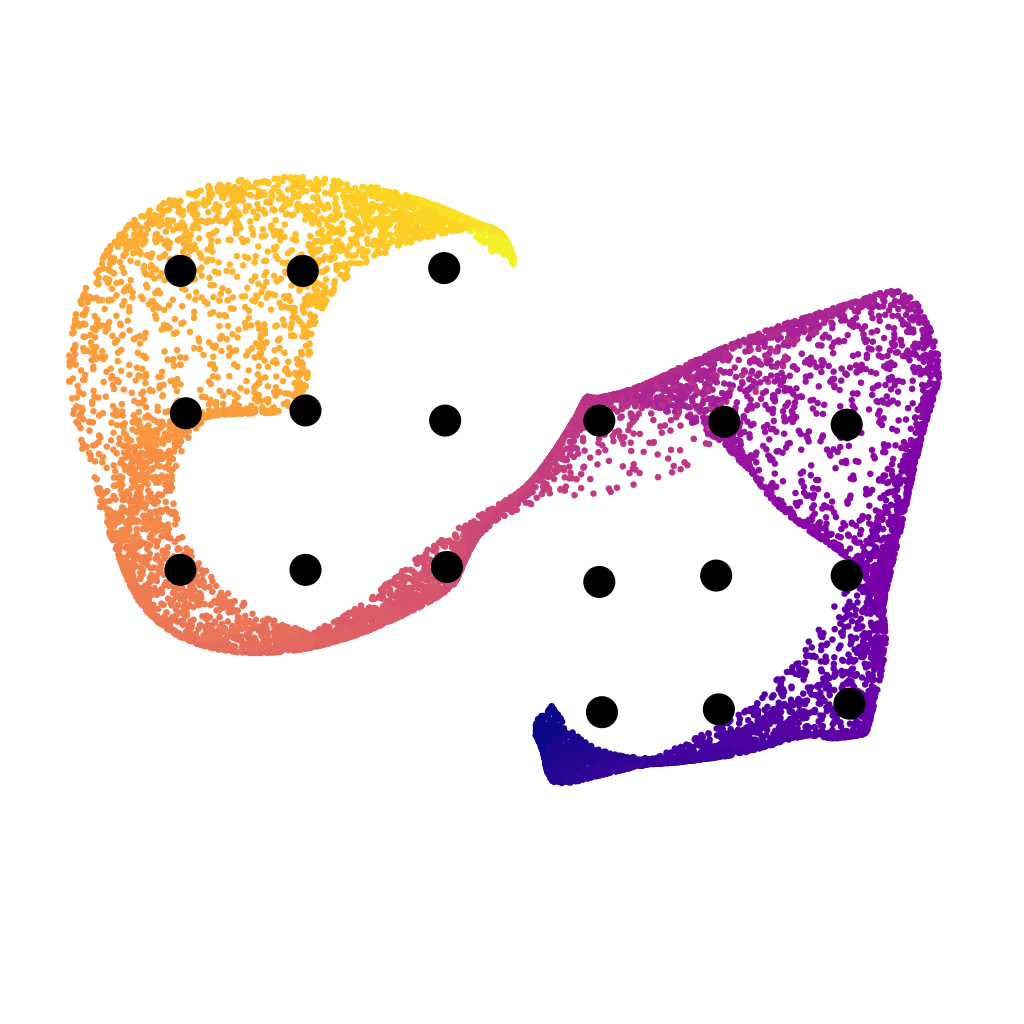
\includegraphics[width=.25\linewidth]{embedsom/pic/S_mid_2d.png}};
% \node[right=of b] (c) {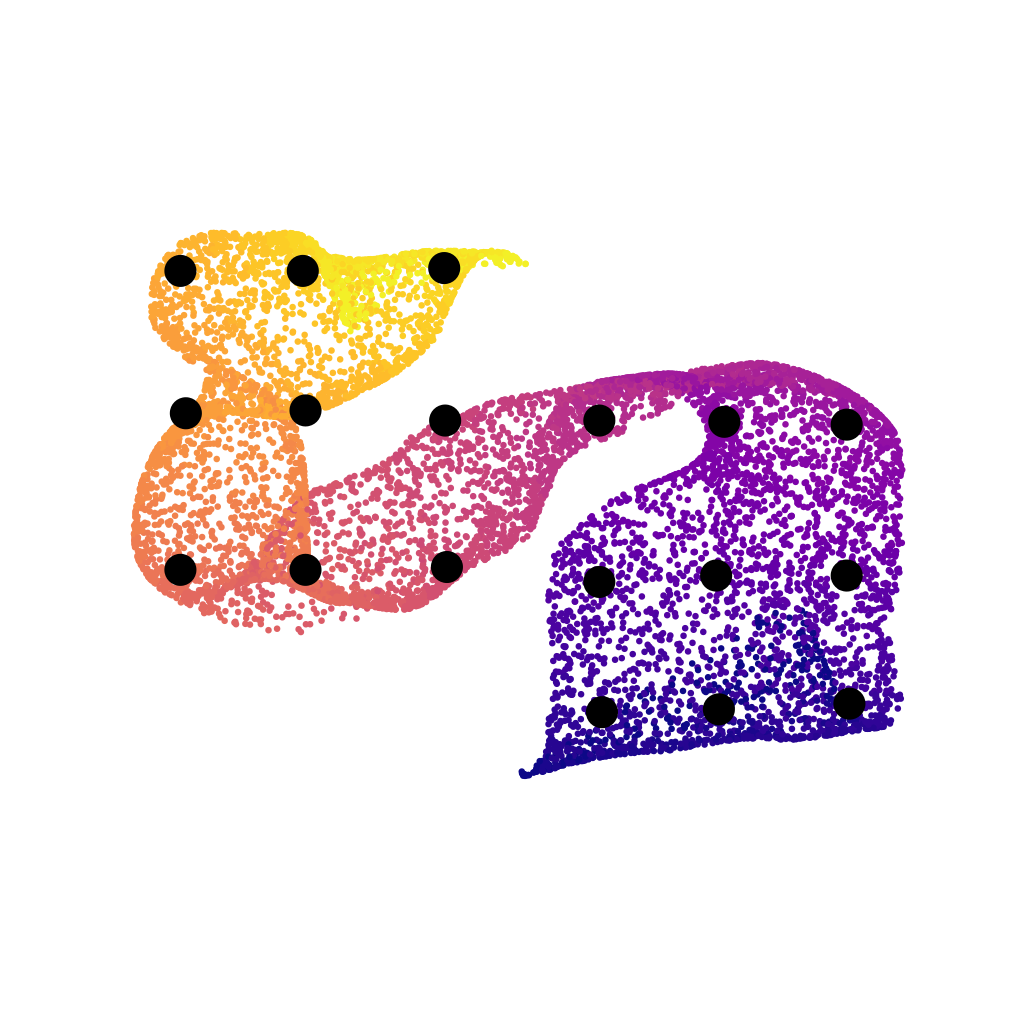
\includegraphics[width=.25\linewidth]{embedsom/pic/S_end_2d.png}};
% \node[below=0pt of a] {$\sigma=1.5$};
% \node[below=0pt of b] {$\sigma=0.8$};
% \node[below=0pt of c] {$\sigma=0.2$};
% \end{tikzpicture}
% \caption{
% Effect of different settings of $\sigma$ SOM training parameter on the output detail, demonstrated on an extruded S-shaped 3D dataset and a custom SOM shape.
% Value of $\sigma$ decreases from left to right, progressively revealing finer details but losing larger-scale structure.
% }
% \label{fig:somsigma}
% \end{figure}
